% INTRODUCTION CONTENT

\section{The cell}
The cell is the smallest unit of life, of which all known living organisms are composed. Every cell houses a plethora of biomolecular processes that allows it to continuously adapt to changes in its environment. Due to the dynamic nature of these processes, it can be very challenging to comprehend the cellular response to a signal. A reductionist approach to understanding a complex biological system is to study the biochemical components of which it is comprised\cite{brigandt_reductionismbiology_2017}.

Recent advances in experimental technologies are playing a crucial role in reductionist biology, allowing to measure the abundance of thousands of different biochemical molecules in tens of thousands of individual cells. With it comes the challenge of analysing large amounts of data that are not easily interpretable by hand. The sheer volume of the data generated from such highly-integrative and high-throughput experiments are not the only reason why they are so challenging to interpret. For instance, the generated data contains high levels of noise arising from inherent biomolecular stochasticity in the cells and from the experimental profiling techniques used, as well as batch effects arising from differences between donors and labs\cite{hon_humancellatlas_2018}. Biologists thus turn to computer scientists
to develop new tools to tackle these problems and help them to extract meaningful biological insights from the data. In this work, incremental contributions were made to the field in order to be able to address the aforementioned problems in a more comprehensive context.

Observing the biomolecular insides of cells can ultimately provide fundamental understanding into the processes that govern these cells and help uncover novel approaches for disease diagnosis, prognosis, and treatment. For example, the Human Cell Atlas (HCA) consortium\cite{regev_humancellatlas_2018} has set out to develop a comprehensive reference map of all the different types of cells in the human body. Experts in the field often metaphorically describe the HCA initiative as aiming to develop a 'Google Maps' of the human body. Even in its infancy, the HCA has profiled 3.8 million cells from 248 donors across 42 labs\cite{humancellatlasconsortium_humancellatlas_2018}, and this number is likely to increase well above one hundred million.

The next part of the chapter highlights several key concepts in both cell biology and computer science, upon which the remainder of this work relies.

\subsection{The origin of life and the RNA world}
The discovery of the double helix shape of deoxyribonucleic acid (DNA)\cite{watson_molecularstructurenucleic_1953} is often considered the pivot point in our understanding of the origin of life and evolution. By now, it is well known that DNA serves as a medium for storing the genetic information required to reproduce a whole organism. With other words, the DNA of an organism contains the complete set of instructions required to build all of the biomolecular machinery present in its body. 

Life (or cells) did not originate from DNA, however. A widely-accepted hypothesis states that life originates from its lesser-known cousin, ribonucleic acid (RNA). According to the RNA world hypothesis\cite{alberts_rnaworldorigins_2002}, the very first primitive cells used RNA both to store genetic information and to perform the chemical reactions required to sustain themselves (Figure \ref{fig:rnaworld}). Only later did cells develop the ability to use the more chemically stable DNA molecules to self-sustain in a process commonly referred to as the central dogma.

\begin{figure}[htb!]
	\centering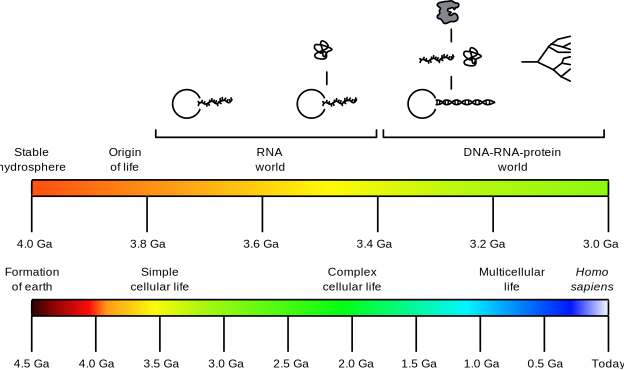
\includegraphics[width=.5\linewidth]{fig/rnaworld} % TODO: change image
	\caption{
		\textbf{RNA world.} The postulated rise and fall of the RNA world during the evolution of life, from early self-replicating RNA to complex, RNA-controlled metabolism, to the invention of translation, followed by diversification of all modern branches of life. Image from Horning (2011)\cite{horning_rnaworld_2011}.
	  \fbox{\color{red} TODO: combine images, rewrite the description.}
	}
	\label{fig:rnaworld}
\end{figure}

The central dogma describes the general flow of genetic information in almost all existing living cells: DNA is decoded to RNA, which in turn encodes proteins\cite{strachan_humanmoleculargenetics_2011}. Main processes involved in the central dogma are \textbf{transcription}, \textbf{splicing}, and \textbf{translation} (Figure \ref{fig:centraldogma}). 

\begin{figure}[htb!]
  \centering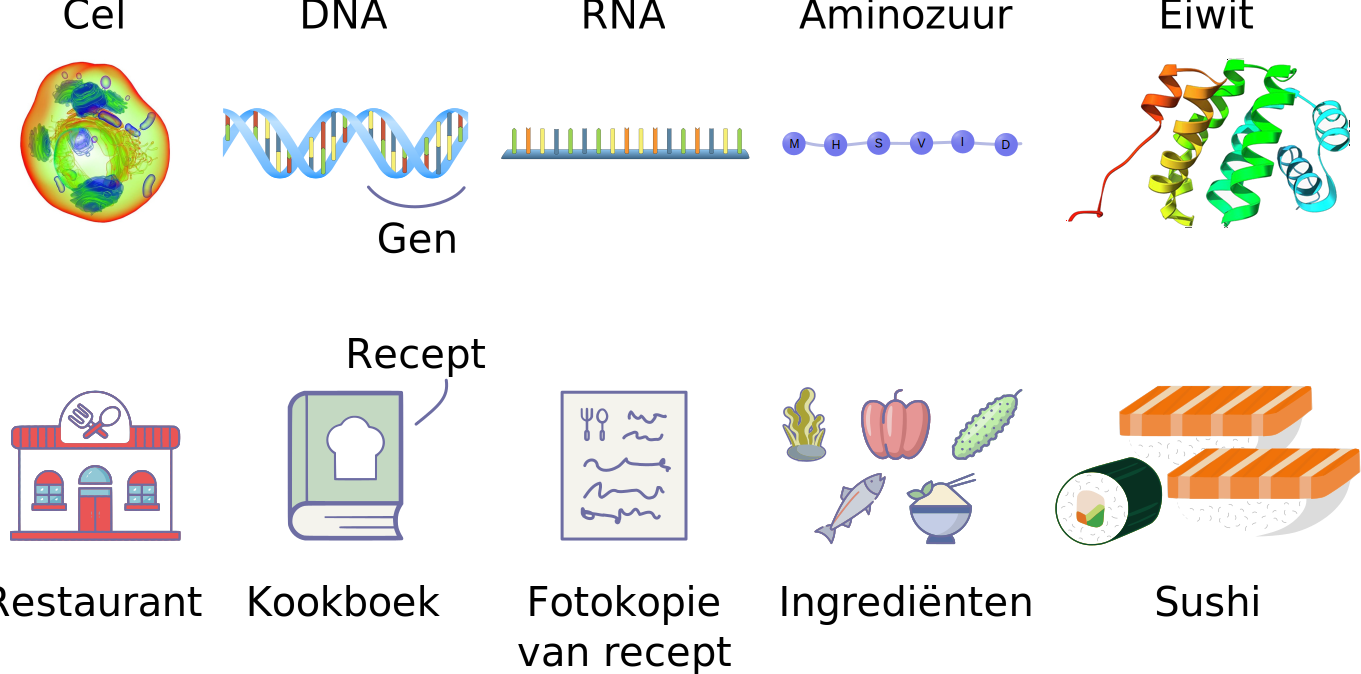
\includegraphics[width=.5\linewidth]{fig/central_dogma} % TODO: change image
  \caption{
    \textbf{Central Dogma.}
    \fbox{\color{red} TODO: combine images, rewrite the description.}
  }
  \label{fig:centraldogma}
\end{figure}

During the process of \textbf{transcription} that takes place in the cell nucleus, a complementary RNA copy is transcribed from the template DNA. The initial RNA transcript is a precursor messenger RNA (pre-mRNA) that needs to undergo series of maturation steps to ultimately form the mature messenger RNA (mRNA). This maturation includes pre-mRNA \textbf{splicing} to remove non-protein coding intervening sequences (the introns) and to join the neighbouring protein-coding sequences (the exons). A single pre-mRNA can be alternatively spliced to generate multiple forms of mRNAs that will result in the production of multiple protein isoforms. This process of alternative splicing is essential to generate more than 100'000 different proteins starting from just 20'000 genes\cite{nilsen_expansioneukaryoticproteome_2010}.
 
The mature mRNA is then transported to the cytoplasm, where it engages with ribosomes to initiate \textbf{translation}. During this highly evolutionary conserved process, a chain of amino acids, known as the protein building blocks, is being synthesised. Each amino acid is specified by three nucleotides (a codon) in the mRNA, according to a nearly universal genetic code. After being released by the ribosomes, the translation product undergoes a variety of chemical modifications to form the final folded protein, the structure of which is determined by the sequence of different amino acids in the chain. In addition, polypeptides may be cleaved to yield more than one active polypeptide product. The structure of a protein determines its functionality, which includes catalysing biochemical reactions, providing structure, and transportation of molecules.


\subsection{Cell types}
\textit{Homo sapiens} like to categorise everything they encounter, and so too have they conceptualised groups of cells called "cell types". The human body contains more than 200 different cell types that are classified into four groups: epithelial, connective, muscle, and nervous. This however, is a major underestimation of the real number of cell types. Neurons, for instance, that are known to be extremely diverse, are estimated to reach numbers above 10,000 different types\cite{strachan_humanmoleculargenetics_2011}.

The concept of cell types eases reasoning and our understanding about many aspects of biology (e.g. the process of cell differentiation, cell-cell communication, cellular response to certain stimuli). Some cells are known to be highly specialised toward performing a particular function (e.g. memory B cells accelerate immune response by remembering previously encountered pathogens), or they can maintain a strong ability to differentiate into other cell types.

One common approach for understanding the functionality of a particular cell is to observe which molecules are present in the cell and to associate those set of molecules with functionality. Taking a snap shot of the protein or RNA transcript content in a particular cell, might already provide us with major insights into its functionality. However, in order to fulfil a particular task, the biochemical machinery of the cell gradually changes over time. Therefore it is highly informative to also consider the transition states between cell types and the dynamic processes involved therein.

\subsection{Cell dynamics and gene regulation}
Cells are dynamic entities that can gradually produce the molecules needed to acquire new functionality. The variation within and between cells happens because of differences in gene expression. The mechanism by which this happens is called gene regulation, and takes place primarily at the level of transcription. According to the needs of a cell, different genes are being transcribed. Housekeeping genes are being expressed in essentially every cell, while other genes are cell type or tissue specific and may be expressed at certain developmental stages\cite{strachan_humanmoleculargenetics_2011}.

% CVC

Some proteins (or other molecules such as micro RNAs) are capable of determining the rate at which a gene is transcribed (transcription rate). Such proteins are called transcription factors (TFs), and the genes they regulate are called their targets. Typically, one TF will regulate the transcription rate of many targets.

Production of a specific molecule might require multiple cascades of gene regulation. The collection of all gene regulatory interactions between transcription factors and targets is called a gene regulatory network (GRN). Studying the active parts of a cell's gene regulatory network can thus reveal which dynamic processes are taking place. 

\subsection{Profiling single cells}
In order to understand a biological process, it is often quite helpful to be able to profile (i.e. observe) the biomolecular components involved therein. The single-cell "omics" technologies which we have at our fingertips today originated from the convergence of two different fields, \emph{"single-cell"} and \emph{"omics"}.

\subsubsection{Single-cell}
The earliest approaches for measuring the abundance of particular molecules in \emph{single cells} used the preferred instrument of every stereotypical biologist: the microscope.
Since it was developed by Coons et al. in 1941, immunohistochemistry (IHC) has been instrumental in visualising antigen-antibody proteins\cite{coons_immunologicalpropertiesantibody_1941}. In many multicellular organisms, antibodies and antigens serve as crucial communication tools as part of the organism's immune system. A cell can present a particular type of antigen on its cell surface, which allows a particular type of antibody to bind to it.

\mycomment{Rephrase the microscope sentence (dino joke?)}

IHC (and many other biotechnologies) visualises antigen-antibody reactions by attaching particular molecules to the antibody, such as an enzyme that catalyses a colour-producing reaction, or a fluorescent chemical compound that can re-emit light upon light excitation. Using different colours (wavelengths) allows measuring expression levels of different antibodies simultaneously. Characterising cells in a quantifiable way is labour intensive; however, since it involves acquiring an image of many cells and drawing a contour around each cell (called cell segmentation). While modern implementations of IHC improve the throughput drastically by using robots to automate the image acquisition and computer software to automate cell segmentation, the procedure is still labour intensive as the robots and computer software still needs to be kept in check.

Flow cytometry\cite{fulwyler_electronicseparationbiological_1965} is a technique which circumvents imaging and segmentation issues by having a steady stream of cells run through a laser and measuring the amount of light scattered from those cells. Flow cytometry technology enables to measure protein expression levels for millions of cells and tens of different antibodies. 

Since IHC and flow cytometry, many new technologies have been developed which allow quantifying expression levels of molecules in single cells (e.g. mass cytometry, single-cell qPCR, FISH). All of these single-cell (non-omics) technologies are limited by the number of different molecules they could measure, however; and thus required handpicking the molecules of interest before performing an experiment, making the experiment biased towards the preconceptions of the experimenter.

\subsubsection{Omics}
On the other side of the spectrum are the so-called "omics" technologies. "Omics"\footnote{The etymology of "omics" is quite interesting\cite{yadav_wholenesssuffixomics_2007}.} is a collective term for profiling all molecules of a particular type in a high-throughput manner. There are many types of "omics", but the most commonly used are the following. In genomics, all of an organism's genes are studied -- its whole genome. Transcriptomics and proteomics study the organisms RNA transcripts and proteins, respectively. A notable downside of traditional omics technologies is that in order to capture enough material an ensemble of cells needs to be profiled, and thus only the average expression levels are returned; thereby granting the technology the name "bulk" omics. If a subset of these cells contains unique patterns in expression levels, this pattern will be masked in the bulk population and is thus undetectable. Specific examples of omics technologies are next-generation sequencing, which can be used to determine the DNA sequence of an organism, and RNA sequencing, which profiles the sequences of RNA transcripts. By mapping the sequences of RNA transcripts to genes in the organisms DNA, a gene expression profile can be obtained.
\mycomment{Demonstrate the masking effect of bulk analyses.}

\subsubsection{Single-cell omics}
Transformative technological advances in microvolume sequencing allowed Tang et al. to analyse the transcriptome at single-cell resolution\cite{tang_mrnaseqwholetranscriptomeanalysis_2009}, thereby bringing single-cell biology and omics together to create single-cell omics (Figure \ref{fig:profiling_convergence}A). During the decade that followed, the number of single-cell omics technologies has skyrocketed, allowing to profile tens of thousands of cells (Figure \ref{fig:profiling_convergence}B) and measuring other levels of information such as proteomic expression levels (Figure \ref{fig:profiling_convergence}C).

\begin{figure}[htb!]
  \centering
  A. 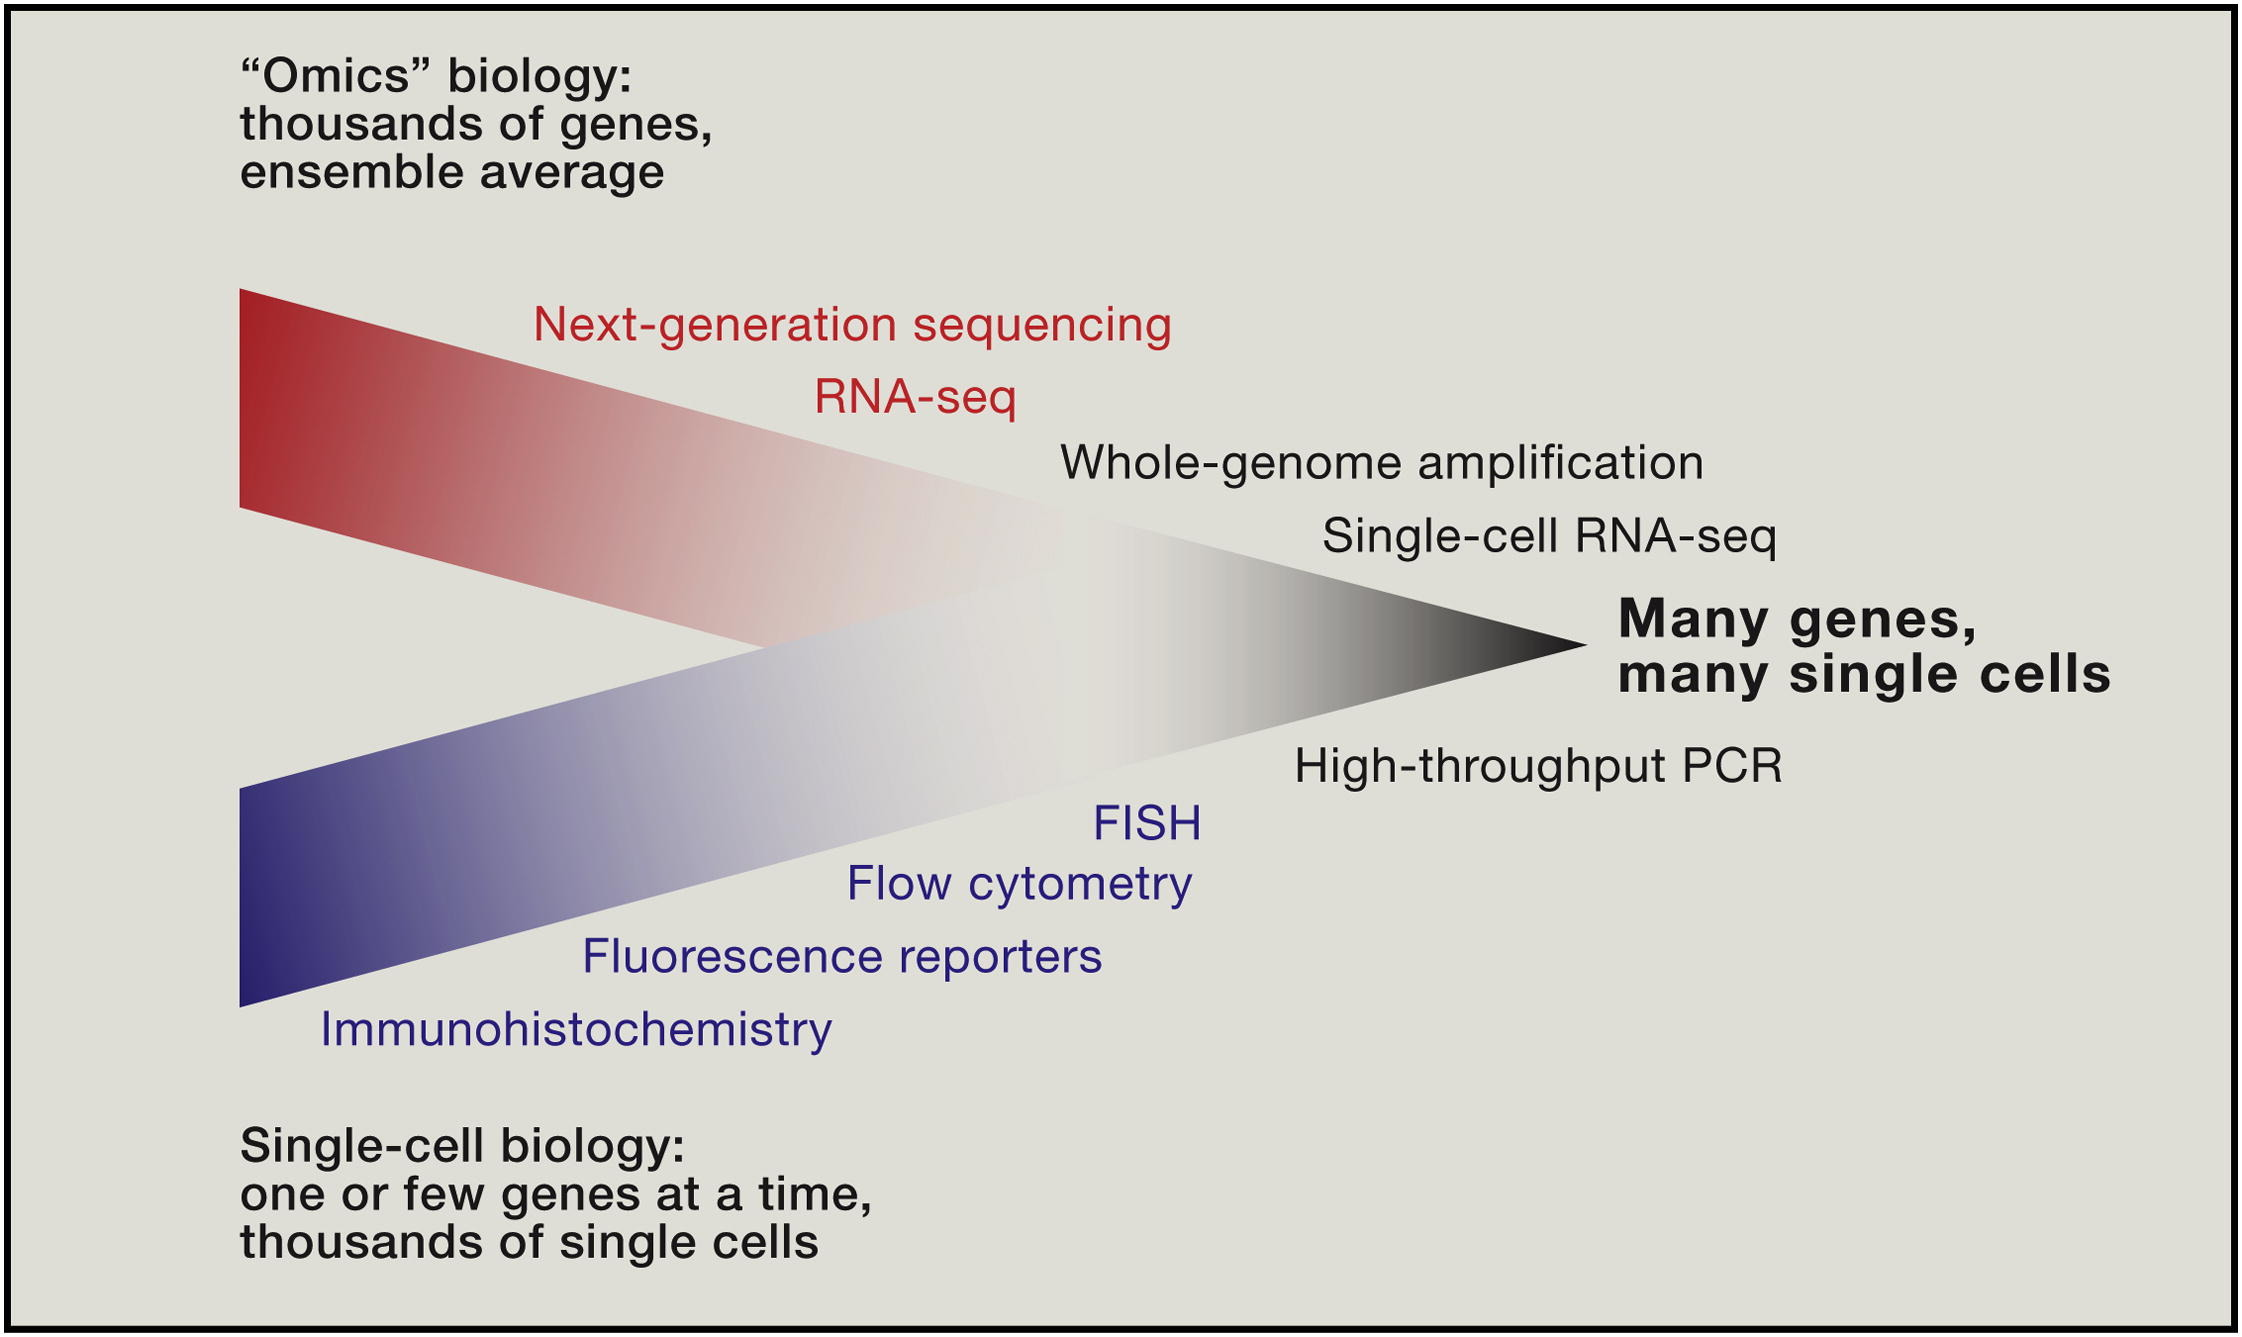
\includegraphics[width=.45\linewidth]{fig/profiling_convergence} 
  % also figure with cell numbers
  C. 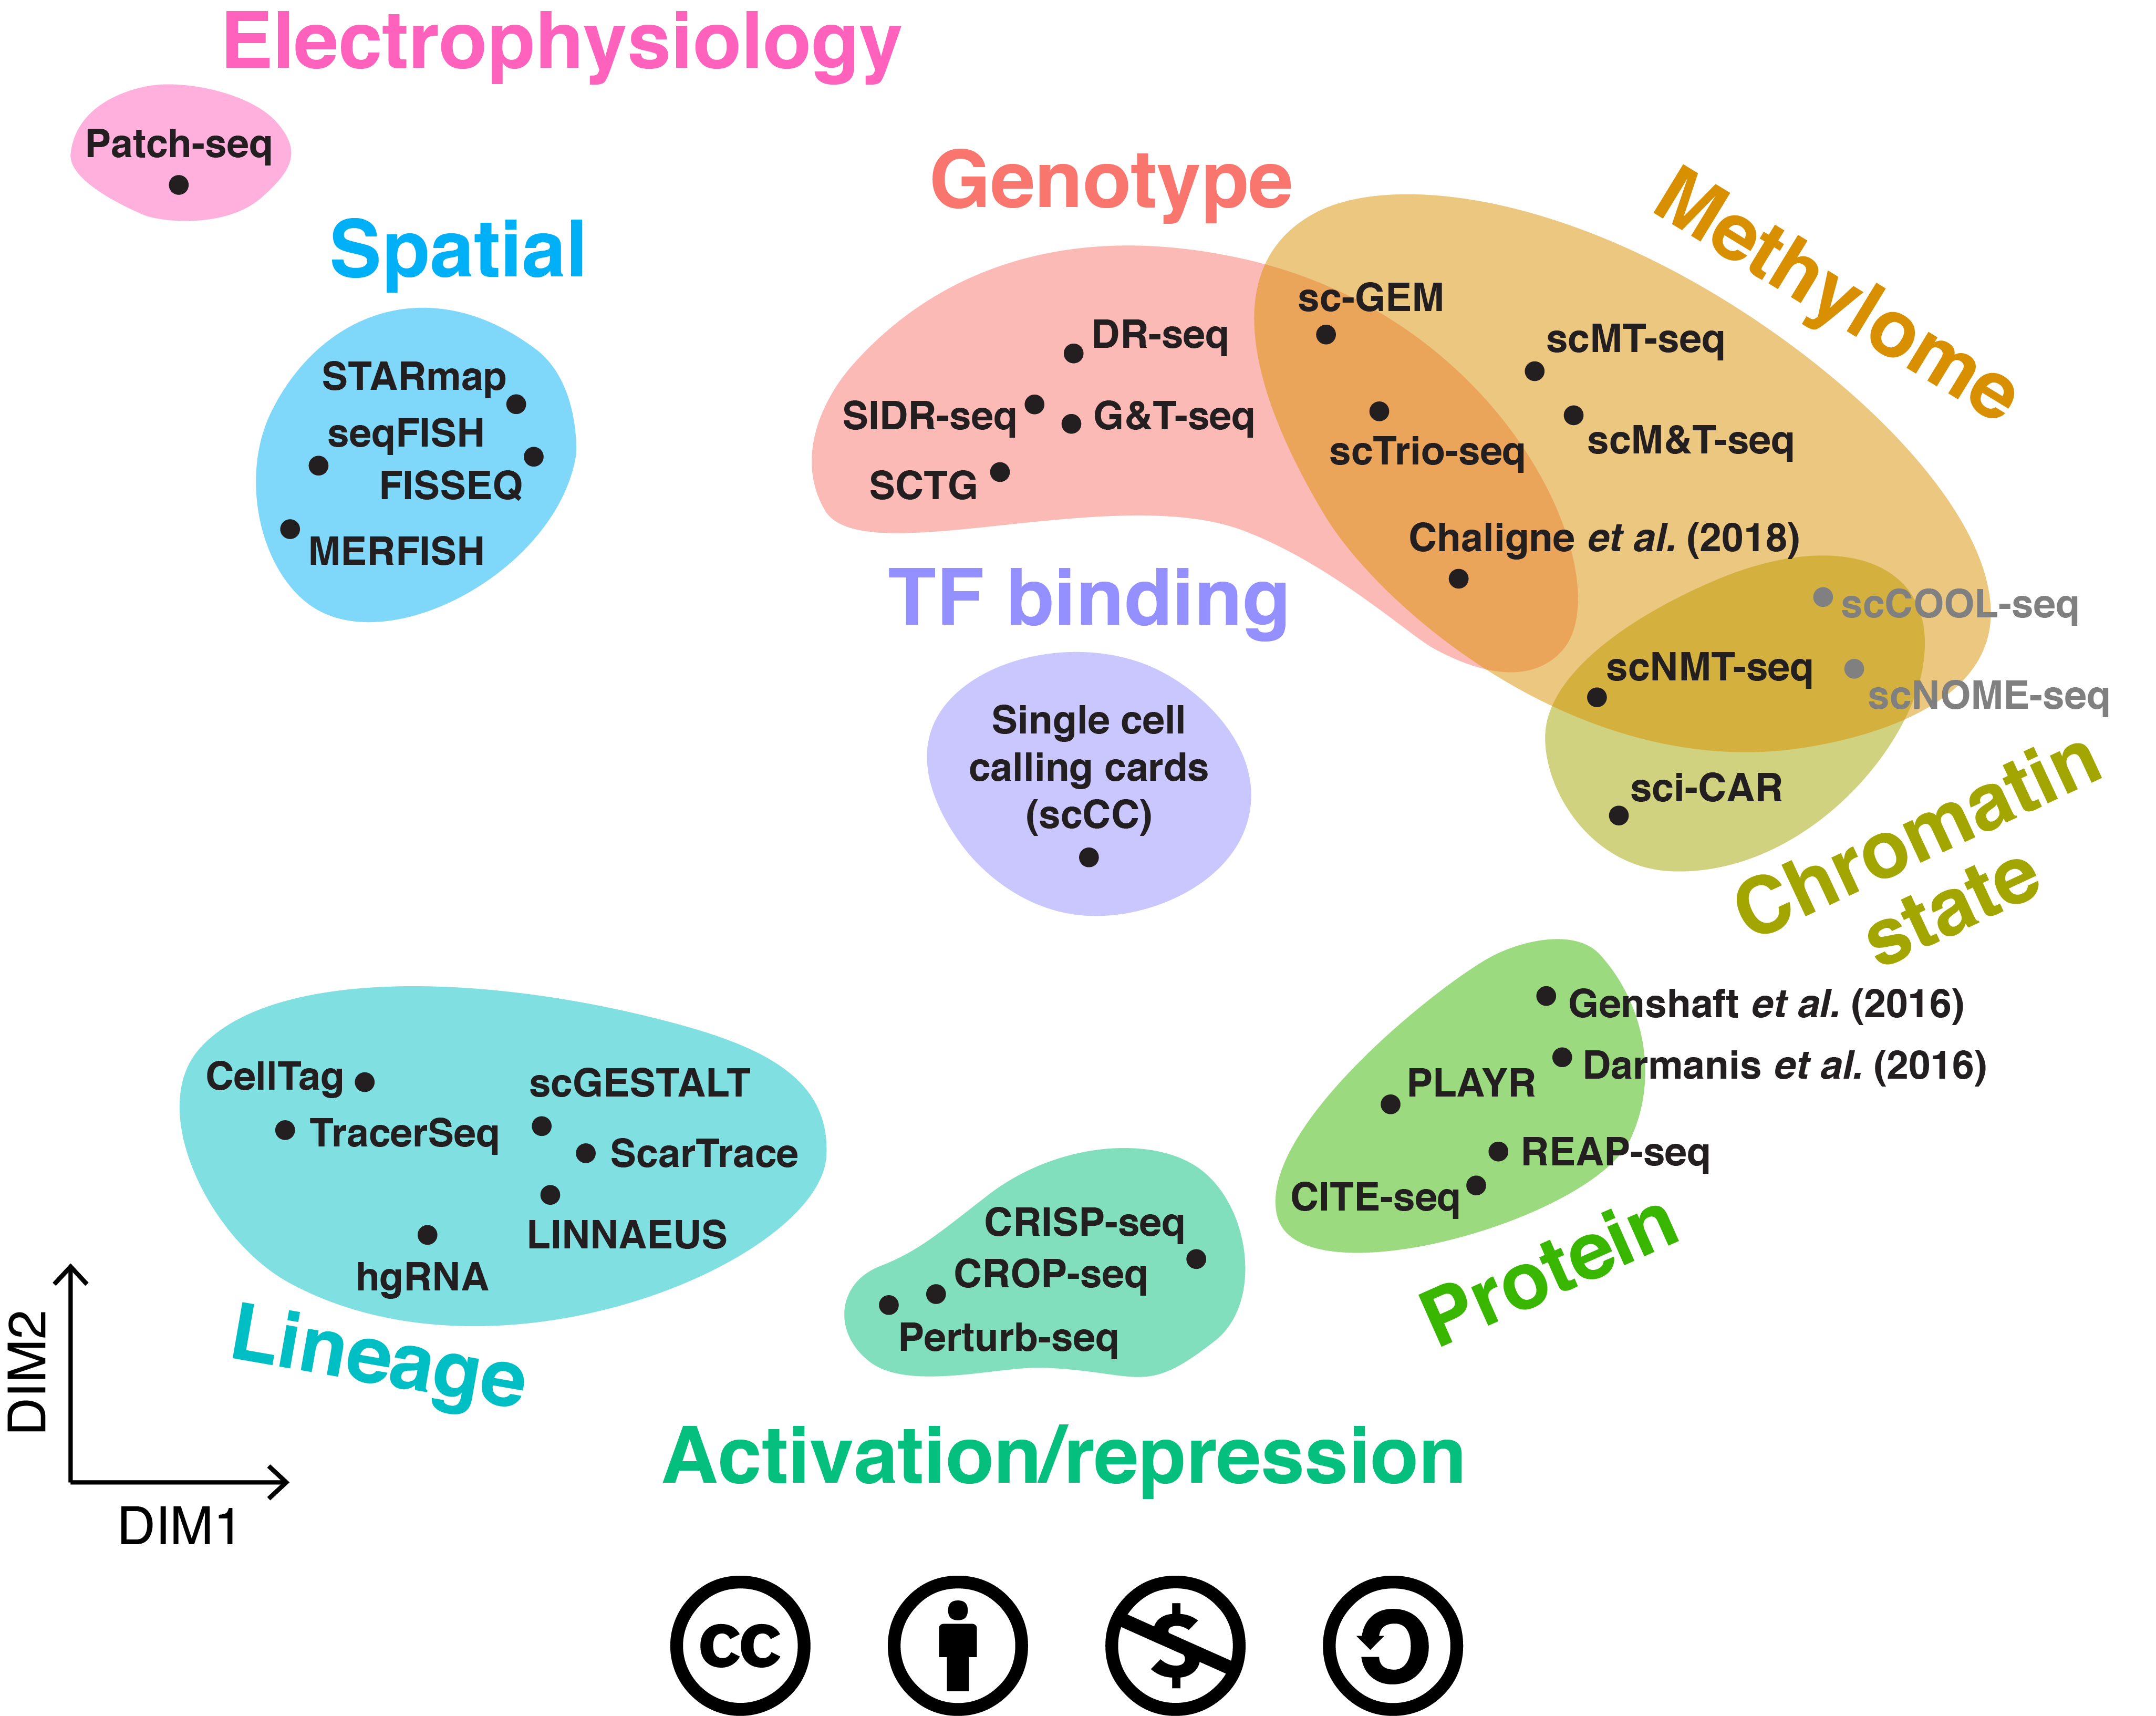
\includegraphics[width=.45\linewidth]{fig/multimodal} 
  \caption{
    A. \textbf{Convergence of "Omics" Biology and Single-Cell Biology.} Technology that allows researchers to obtain genome-wide information from single cells is extending the boundaries of a field that has thus far been limited to the analyses of a select gene in eukaryotes. Image from Junker and van Oudenaarden (2014)\cite{junker_everycellspecial_2014}. 
    B. Cell numbers vs. gene count over time.
    C. scmultiomics\cite{moudgil_multimodalscrnaseq_2019}. 
    \fbox{\color{red} TODO: combine images, rewrite the description.}
  }
  \label{fig:profiling_convergence}
\end{figure}

The rapidly advancing field of single-cell omics harbours exceptional opportunities to discover new aspects of biology and redefine existing knowledge. Some of these opportunities lie in efforts like the Human Cell Atlas. The HCA consortium has set out to redefine all human cell types in terms of their gene expression and location, and the developmental trajectories connecting the different cell types. As part of this endeavour, the consortium will likely profile the whole transcriptomes tens or even hundreds of millions of cells. 

\section{Computational tools}
The new types of analyses permitted by single-cell omics harbour exceptional opportunities to discover new aspects of biology and redefine existing knowledge (Figure \ref{fig:comp_tools}A). These include the following categories\cite{zappia_exploringsinglecellrnaseq_2018}.
\begin{itemize}
	\item \textbf{Data imputation}: \ldots.
	\item \textbf{Data integration}: \ldots.
	\item \textbf{Clustering}: \ldots.
	\item \textbf{Dimensionality reduction}: providing a visual and informative overview of a given dataset.
	\item \textbf{Trajectory inference}: identifying and characterising transitions between different cellular states.
	\item \textbf{Trajectory alignment}: \ldots.
	\item \textbf{Network inference}: inferring gene regulatory interactions between transcription factors across individual cells.
\end{itemize}
\mycomment{To do: write a section for each of these categories.}

Developing new computational tools to perform these analyses has proven challenging for two main reasons\cite{stegle_computationalanalyticalchallenges_2015, yuan_challengesemergingdirections_2017, chen_singlecellrnaseqtechnologies_2019}. Firstly, single-cell omics data suffers from hitherto unseen noise characteristics, including high dropout rates and high levels of transcriptional stochasticity. In addition, a low abundance of single-cell omics data that can be used as a ground-truth obstruct quantitative evaluation of such methods. 


\begin{figure}[htb!]
  \centering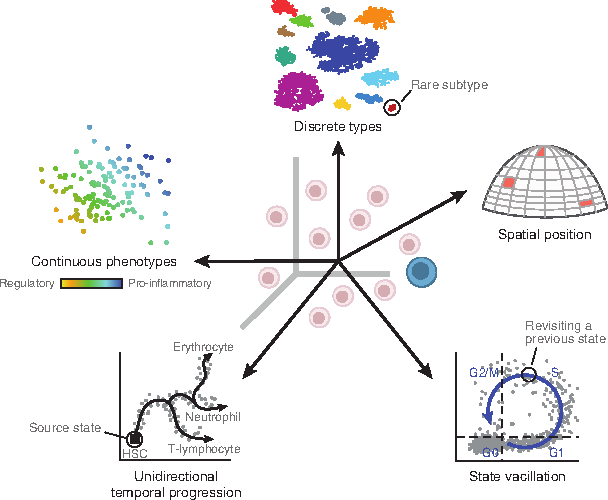
\includegraphics[width=.5\linewidth]{fig/singlecell_tools}
  \centering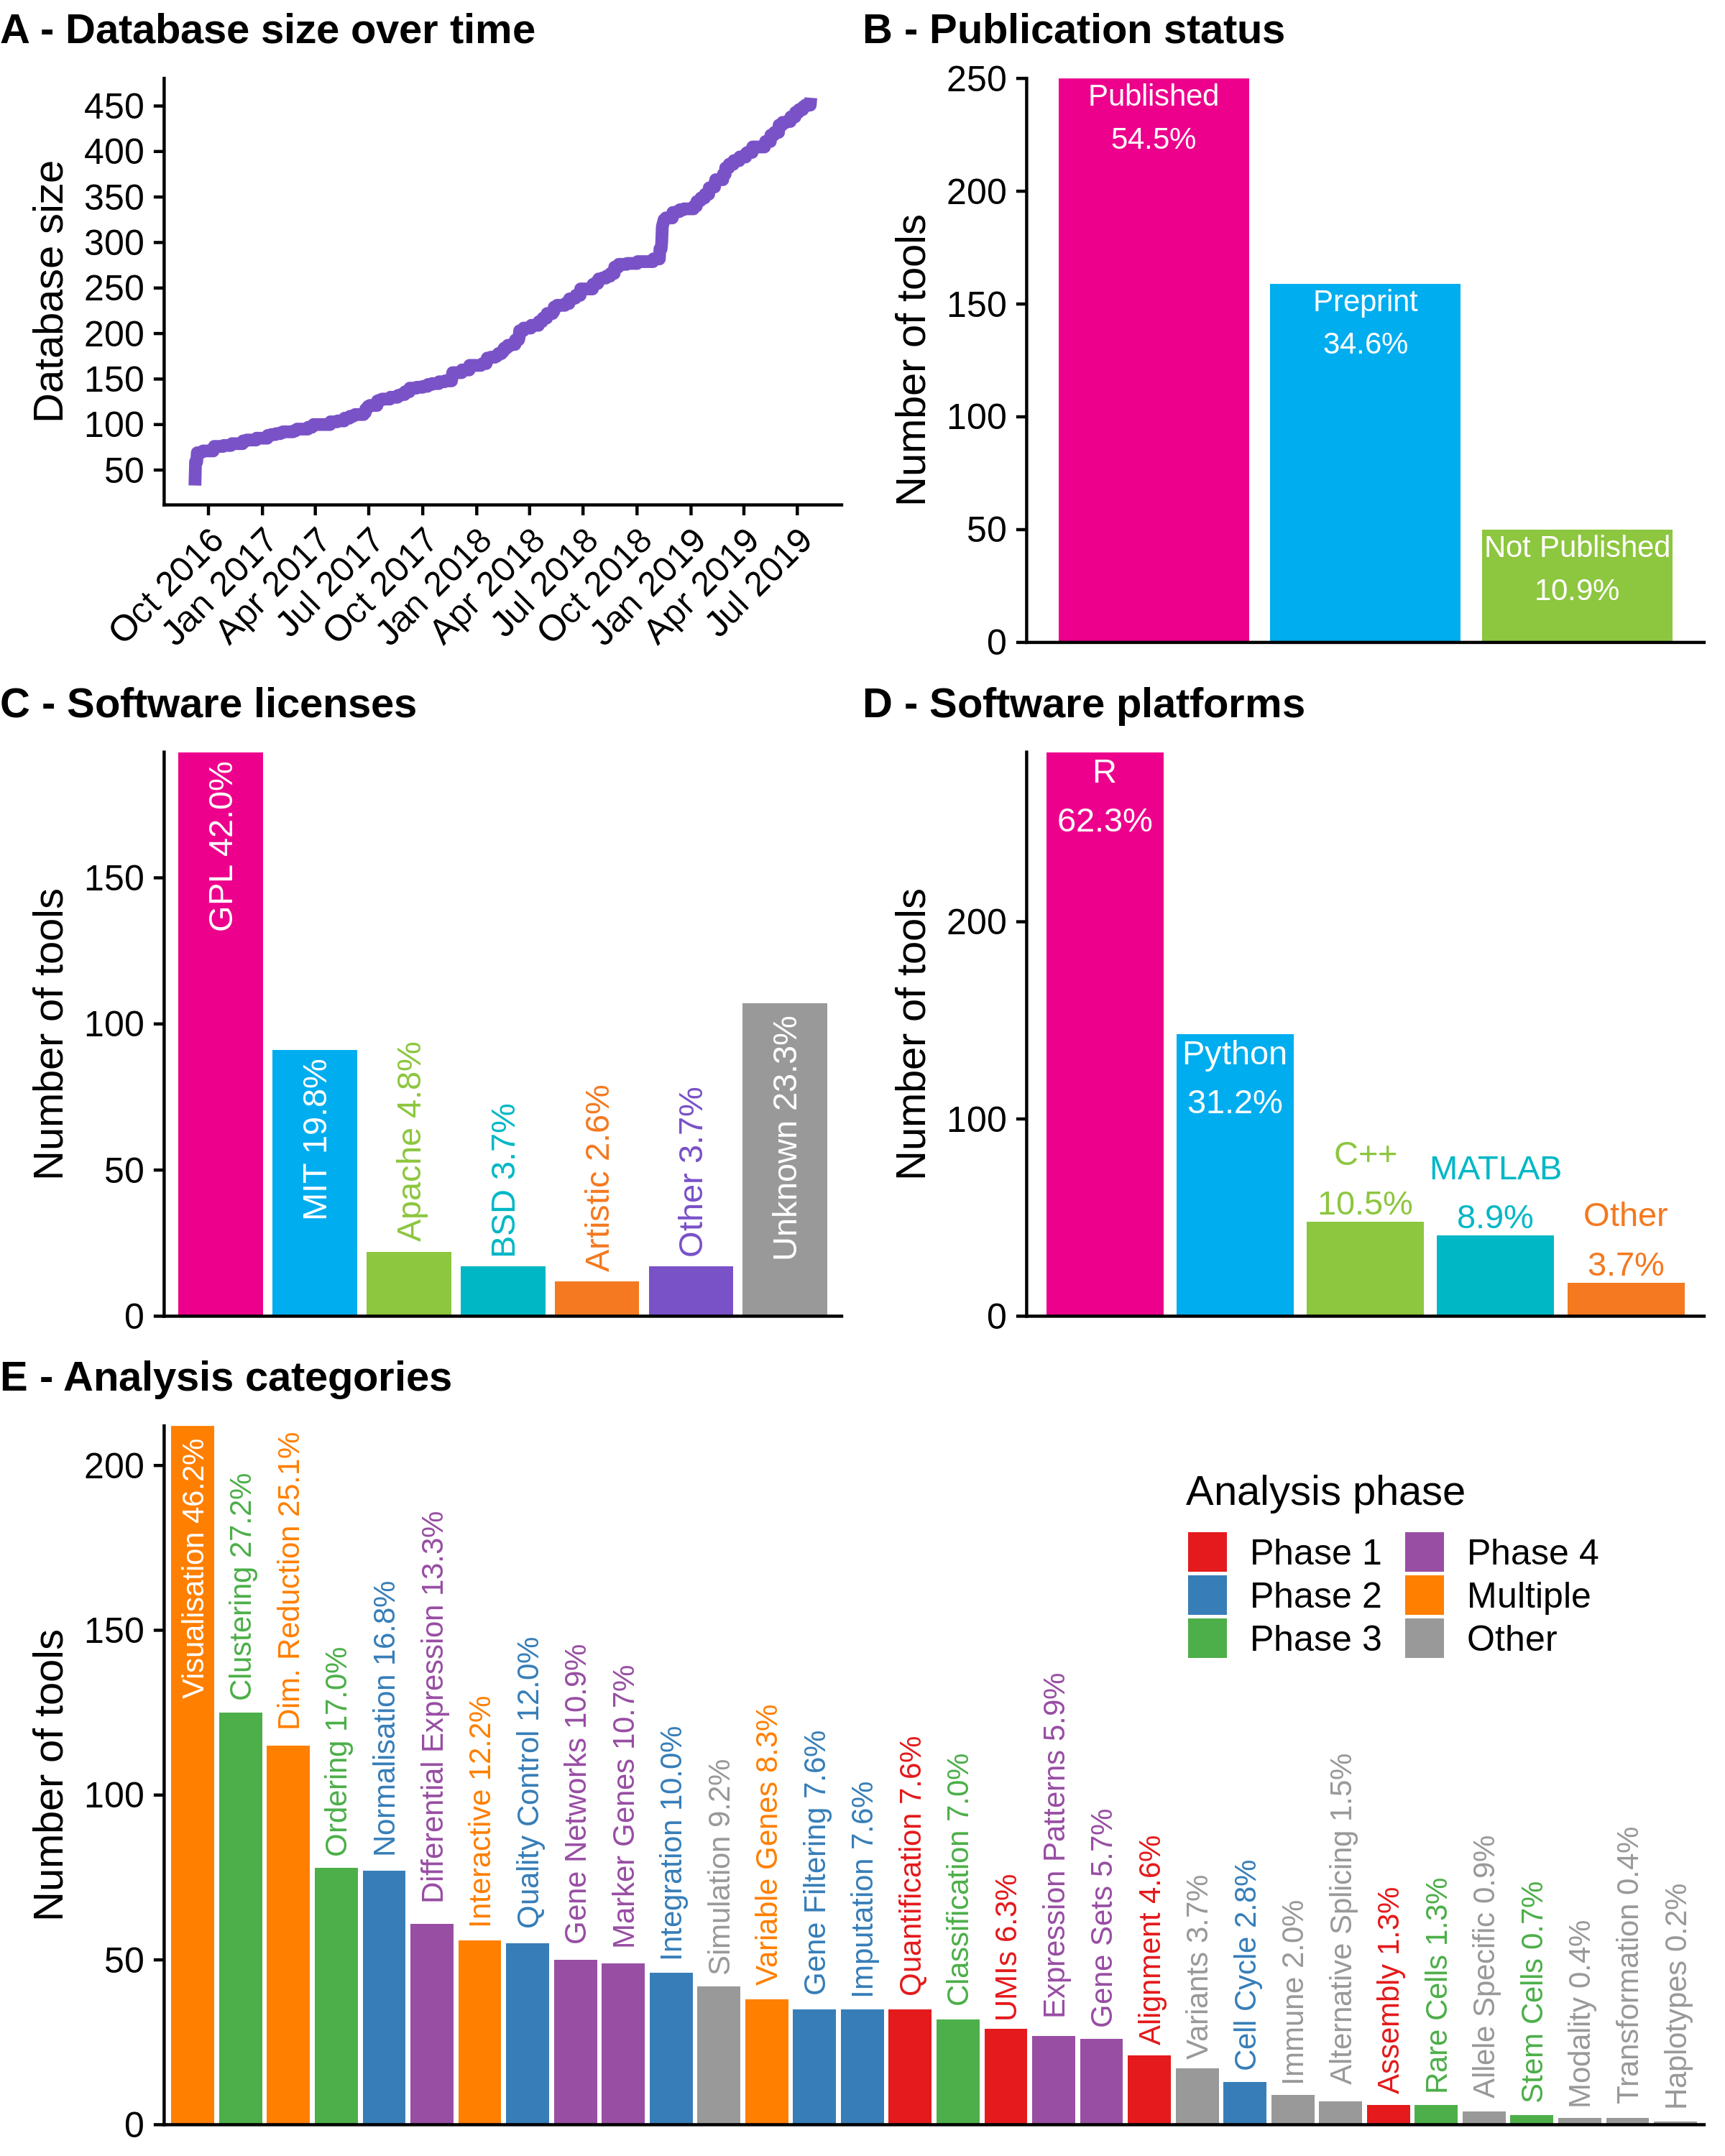
\includegraphics[width=.3\linewidth]{fig/scrnatools}
  \caption{\textbf{A. Single-cell omics allows for many new types of computational approaches.} Figure adapted from Wagner et al. (2016)\cite{wagner_revealingvectorscellular_2016}.
    B. Zappia et al. (2018)\cite{zappia_exploringsinglecellrnaseq_2018}.
    \fbox{\color{red} TODO: combine images, rewrite the description.}
  }
  \label{fig:comp_tools}
\end{figure}

\subsection{Dimensionality reduction}
Single-cell omics datasets typically have too many dimensions (features) in order to be easily interpretable by humans and even by most computational tools. 
Dimensionality reduction (DR) methods transform high-dimensional data into a meaningful representation with fewer dimensions. It is important to note that its usage depends on the target audience: for humans -- to visualise data in a 2-D plane to aid with interpretation by humans, or for computers -- to construct a denser representation of the data such that it mostly contains the same information but with fewer dimensions.

There are many ways of classifying DR methods\cite{engel_surveydimensionreduction_2012}, but this work will use the following main categories: feature projection-based and manifold learning. 
Projection-based DR methods aim to perform a linear transformation of the data while preserving the pairwise distances between samples as much as possible. Examples of commonly used projection-based DR methods in single-cell omics are PCA and MDS. 
Manifold learning methods are methods which reconstruct a higher-order structure in the original space (e.g. a graph or a grid), visualising the structure in a lower-dimensional space, and mapping the original samples to the lower-dimensional space. Manifold learning can be an iterative optimisation process using a predefined criterion. Examples of manifold learning techniques are t-SNE, Diffusion Maps and UMAP. 

\mycomment{This section is not very interestingly written}

\subsection{Trajectory inference}
Single-cell omics data provide new opportunities for studying cellular dynamic processes, such as the cell cycle, cell differentiation and cell activation\cite{tanay_scalingsinglecellgenomics_2017,etzrodt_quantitativesinglecellapproaches_2014}. 
Trajectory inference (TI) is a new category of computational tools used to offer an unbiased and transcriptome-wide understanding of a dynamic process\cite{tanay_scalingsinglecellgenomics_2017,cannoodt_computationalmethodstrajectory_2016}. 

Technological advancements in single-cell omics allow studying a dynamic process in a high-throughput manner. 
This raises concerns regarding biological fundamentals, such as how to define cell types or transitions between them\cite{etzrodt_quantitativesinglecellapproaches_2014,tanay_scalingsinglecellgenomics_2017}. 
Trajectory inference (TI) methods aim to give insight into a dynamic process by inferring a trajectory from omics profiles of cells in which the dynamic process takes place\cite{cannoodt_computationalmethodstrajectory_2016}. 
TI has two objectives: to reconstruct the topology of the dynamic process (e.g. is it linear, cyclical, bifurcating), and to determine the position of each cell along the topology. Some TI methods assumes that the user knows the topology beforehand and only focuses on ordering the cells along a predefined topology.

The dataset can be a single snapshot of a mixture of cells in different stages, or a set of samples collected at different time points (Figure \ref{fig:trajectory_inference}A). Typically, TI methods first analyse similarities between cells, optionally infer the topology of the underlying process, and finally order cells along that trajectory (Figure \ref{fig:trajectory_inference}B). The second step can be optional, as some methods assume a specific topology beforehand.
TI methods allow the identification of new subsets of cells, delineation of a differentiation tree, and characterisation of the main driver genes along a state transition (Figure \ref{fig:trajectory_inference}C). Current applications of TI focus on specific subsets of cells, but ongoing efforts to construct transcriptomic catalogs of whole organisms\cite{regev_humancellatlas_2017,han_mappingmousecell_2018,schaum_singlecelltranscriptomics20_2018} underline the urgency for accurate, scalable\cite{aibar_scenicsinglecellregulatory_2017,angerer_singlecellsmake_2017} and user-friendly TI methods.

\begin{figure}[htb!]
  \centering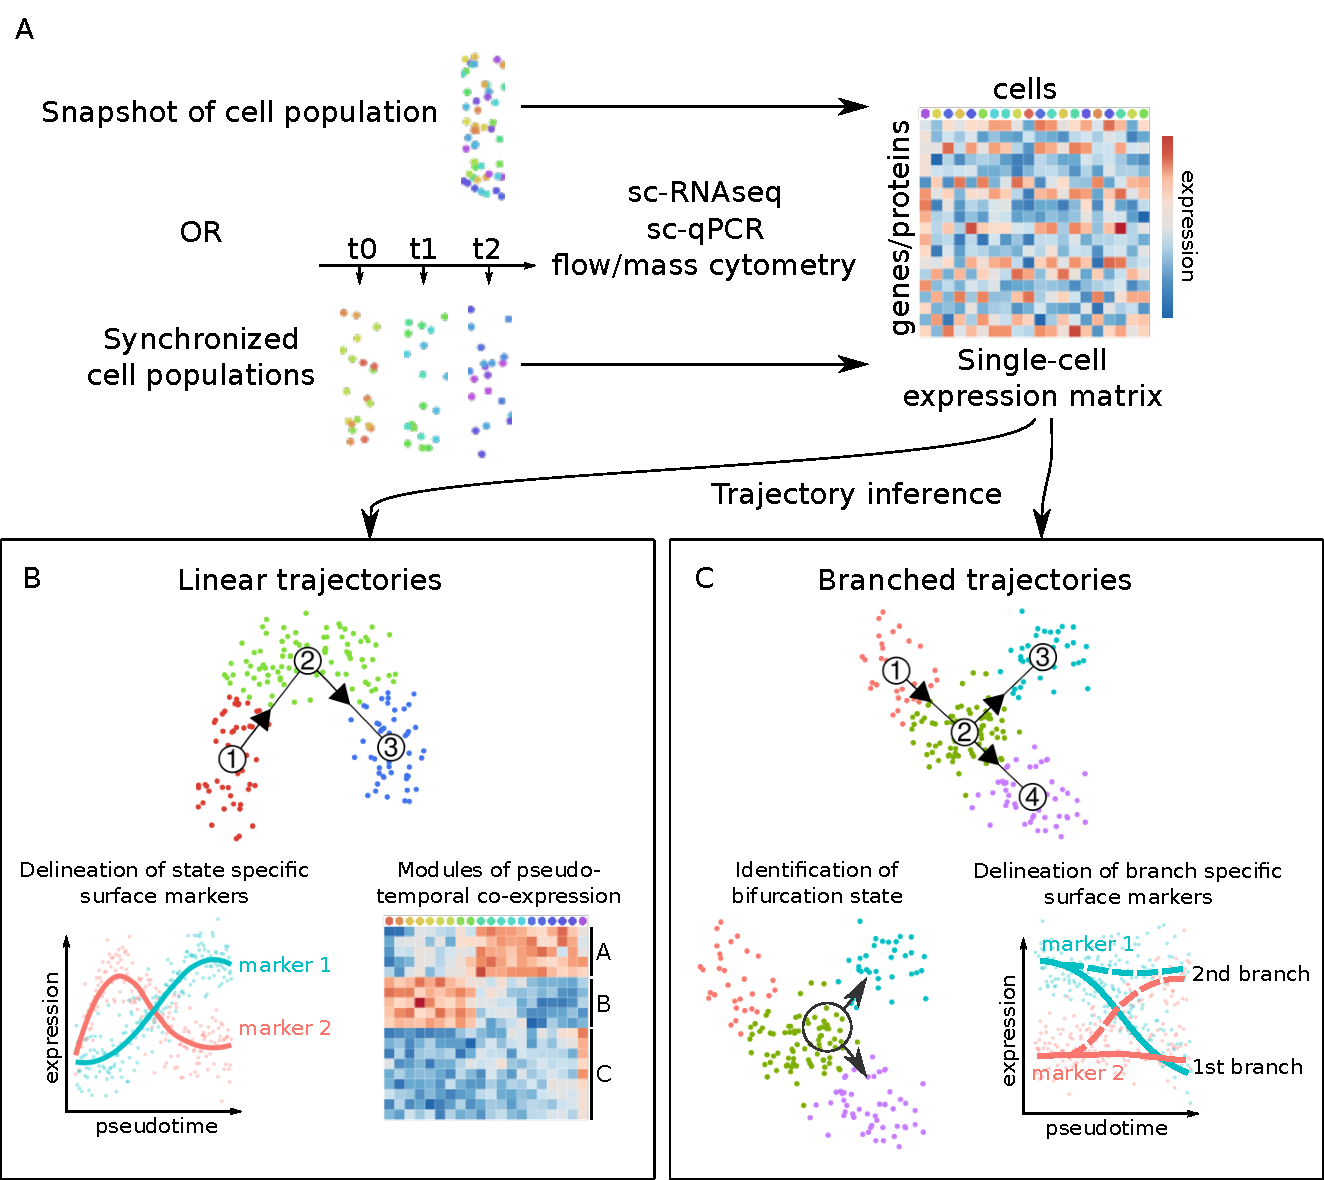
\includegraphics[width=\Largefigure]{fig/trajectory_inference_slim} % TODO: Update figure to match text!!!!
  \caption{
    Applications of single-cell trajectory inference methods. (A) Single-cell omics data appropriate for TI can be both obtained from an unsynchronised population of single cells (snapshot data) but also from synchronised cell populations. (B) UPDATE! (C) UPDATE!
  }
  \label{fig:trajectory_inference}
\end{figure}

\mycomment{Could still expand this section with pieces from the EJI paper, though it needs to be adapted strongly.}

\subsection{Network inference}
Gene regulatory network inference, or network inference (NI) for short, is a type of computational analysis where thousands of transcriptomic profiles are analysed together in order to infer the regulatory interactions between transcription factors and genes. This topic already received much attention with the advent of bulk omics (before single-cell omics). These efforts culminated in several DREAM competitions assessing the performance of 29 different NI methods\cite{marbach_revealingstrengthsweaknesses_2010, marbach_wisdomcrowdsrobust_2012}. 

After the last DREAM competition, it seemed that interest in NI methodology had declined. After all, NI on bulk omics profiles suffered from several crucial issues. As mentioned previously, bulk profiles are generated by pooling together the RNA transcripts of a supposedly homogeneous population of thousands of cells. Since the expression values are averaged over the whole population, incorrect assumptions on the homogeneity of the pooled cells may lead to the masking of relevant expression patterns in rare cell populations (Figure \ref{fig:bulk_vs_singlecell}). Besides, NI methods rely on a diverse set of time-series and perturbation experiments in order to reliably identify causal regulatory interactions. Such experiments are expensive and time-consuming, and an inaccurate selection of time points might result in crucial intermediate stages being missed.

\begin{figure}[htb!]
  \centering
  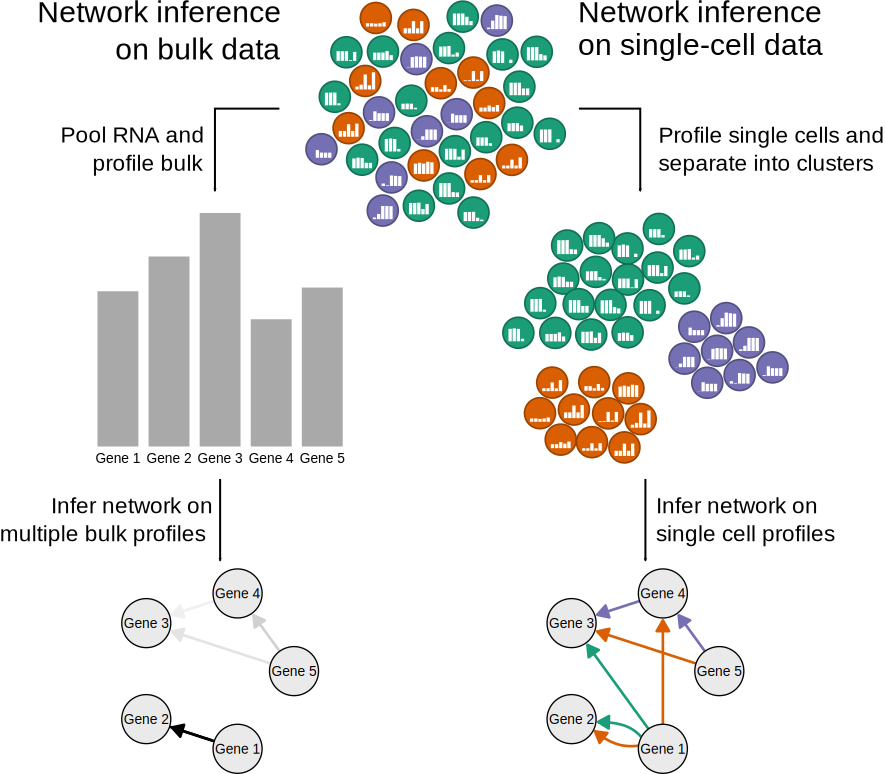
\includegraphics[width=\Largefigure]{fig/ni_bulk_vs_sc}
  \caption{Bulk expression data return the average expressions of genes among large numbers of cells. In order to infer regulatory networks from this type of data, multiple bulk profiles (resulting from time series or perturbation experiments) are required. On the other hand, sequencing the transcriptome at the single-cell level uncovers the high variability among cells, providing the necessary information to infer gene regulatory networks directly.} % TODO: update label
  \label{fig:bulk_vs_singlecell}
\end{figure}

The advent of single-cell omics has made scientists wonder whether now is the time to revisit network inference\cite{stegle_computationalanalyticalchallenges_2015}. 
One of the main advantages of single-cell omics is the ability to quantify the exact cellular state of thousands of cells per experiment. The heterogeneity between cells caused by naturally occurring biological randomness\cite{padovan-merhar_usingvariabilitygene_2013} can be exploited to infer regulatory interactions between TFs and their target genes at much lower costs (see Figure \ref{fig:bulk_vs_singlecell}).
In this setting, heterogeneity in the cell population eases network inference, rather than mask condition-specific expression patterns in regulatory interactions.

\section{Research context and objectives}
Recent technological advancements in profiling single cells are having significant repercussions in many fields of biology. Profiling thousands of individual cells in a genome-wide manner provides opportunities to study cell heterogeneity and dynamics, for example inferring mechanisms for cellular development or intercellular communication. 
Hundreds of new software tools were developed\cite{zappia_exploringsinglecellrnaseq_2018} to perform these new types of analyses, or to fit existing analytical tools to deal with new data characteristics (e.g. differential expression, dimensionality reduction, normalisation). 

One major shortcoming during the advent of single-cell omics was that majority of the newly developed computational tools were not quantitatively and comparatively evaluated. Rather, they relied on anecdotal evidence to demonstrate its usefulness. This issue is not the result of the tool developer's malevolence, but instead of the lack of data required to perform such comprehensive benchmarks.
%TODO: also mention guidelines for users.

Uncontrolled development of software tools without comprehensive benchmarking poses serious problems. 
For one, it slows down scientific progress. Every end-user needs to make a large commitment researching the domain in order to make an informed decision of which tool to use, or risk a higher incidence of false positive discoveries (either way, valuable resources are being wasted). In addition, it also negatively impacts the credibility of the field, thus discouraging potential users or researchers from entering.

In this work, we aim to speed up scientific progress in single-cell omics by providing tools both for end-users and developers alike. For developers of computational approaches, we provide tools and guidelines for benchmarking their method on real and synthetic data. For end-users we develop new tools and guidelines for analysing dynamic processes by inferring trajectories and gene regulatory networks. These contributions are discussed in the following chapters:

\begin{itemize}
  \item We develop benchmarking strategies for assessing the performance of computational tools constrained by low availability of novel types of real single-cell data (Chapter~\ref{chap:dyngen}). \textit{In silico} simulations of individual cells are used to help kick-start emerging domains much more safely and allow anticipation of future technological developments by already developing computational tools.
  \item We apply this strategy to perform a comparison of TI methods (Chapter~\ref{chap:dynbenchmark}). Trajectory inference is one of the largest categories of all the novel single-cell omics tools, yet a comprehensive and quantitative study of the advantages and disadvantages of the numerous tools was hitherto lacking. We provide a set of guidelines for end-users wishing to infer trajectories. We also make our pipeline, datasets, metrics, and containerised wrappers of TI methods publicly available for developers to use.
  \item We developed dyno, a toolkit to easily infer, visualise and interpret single-cell trajectories using more than 50 different TI methods (Chapter~\ref{chap:dyno}). dyno provides downstream analysis such as: visualising a trajectory in a low-dimensional space or a heatmap, detecting genes differentially expressed at different stages of the tragectory, comparing multiple trajectories in a common dimensionality reduction, and manipulating the trajectory (e.g. adding directionality or adding annotation).
  \item We introduce a novel TI method specialised in inferring linear trajectories (Chapter~\ref{chap:scorpius}). Despite linear TI being the most simple but commonly used form of trajectory inference, the benchmark demonstrated that most TI methods are not capable of producing accurate models of linear datasets.
  \item We invent a new type of NI method capable of inferring the GRN of individual cells (Chapter~\ref{chap:bred}). We demonstrate this <yadeyade .. fill in when the chapter is actually written.>
  \item Every NI method has certain topological biases. We provide a tool for analysing the topological properties of large, evolving networks and use this to iteratively optimise GRN predictions (Chapter~\ref{chap:incgraph}).
  \item We discuss reproducibility problems of TI methods due to low rates of quantitative self-assessment (Chapter~\ref{chap:selfassessment}). We provide solutions for different causal reasons for this phenomenon in order to spur developers to perform more self-assessments.
  \item Finally, we summarise our experience in benchmarking computational methods in a list of essential guidelines (Chapter~\ref{chap:guidelines}).
\end{itemize}


\section{List of contributions}

\subsection{First-author publications}

\begin{itemize}
  \item \textbf{Cannoodt R} *, Saelens W *, Saeys Y. Computational methods for trajectory inference from single-cell transcriptomics. European journal of immunology. 2016 Nov;46(11):2496-506.
  \item \textbf{Cannoodt R}, Ruyssinck J, Ramon J, De Preter K, Saeys Y. IncGraph: Incremental graphlet counting for topology optimisation. PloS one. 2018 Apr 26;13(4):e0195997.
  \item Saelens W *, \textbf{Cannoodt R} *, Todorov H, Saeys Y. A comparison of single-cell trajectory inference methods. Nature biotechnology. 2019 May;37(5):547.
  \item \textbf{Cannoodt R}, Saelens W, Sichien D, Tavernier S, Janssens S, Guilliams M, Lambrecht B, De Preter K, Saeys Y. SCORPIUS: Fast, accurate, and robust single-cell pseudotime. In preparation.
  \item \textbf{Cannoodt R} *, Saelens W *, Saeys Y. dyngen: Simulating developing single cells. In preparation.
  \item \textbf{Cannoodt R} *, Saelens W *, Saeys Y. dyno: A toolkit for inferring, visualising, and interpreting trajectories. In preparation.
  \item \textbf{Cannoodt R}, Saelens W, Saeys Y, De Preter K. bred: Inferring single cell regulatory networks. In preparation. \fbox{\color{red}order authors?}
  \item \textbf{Cannoodt R}, Saelens W, Saeys Y. Self-assessment in trajectory inference. In preparation.
 \end{itemize}

*: Equal contribution.

\subsection{Co-author publications}
\begin{itemize}
  \item Decock A, Ongenaert M, \textbf{Cannoodt R}, Verniers K, De Wilde B, Laureys G, Van Roy N, Berbegall AP, Bienertova-Vasku J, Bown N, Clément N. Methyl-CpG-binding domain sequencing reveals a prognostic methylation signature in neuroblastoma. Oncotarget. 2016 Jan 12;7(2):1960.
  \item Van Cauwenbergh C, Van Schil K, \textbf{Cannoodt R}, Bauwens M, Van Laethem T, De Jaegere S, Steyaert W, Sante T, Menten B, Leroy BP, Coppieters F. arrEYE: a customized platform for high-resolution copy number analysis of coding and noncoding regions of known and candidate retinal dystrophy genes and retinal noncoding RNAs. Genetics in Medicine. 2017 Apr;19(4):457.
  \item Claeys S, Denecker G, \textbf{Cannoodt R}, Kumps C, Durinck K, Speleman F, De Preter K. Early and late effects of pharmacological ALK inhibition on the neuroblastoma transcriptome. Oncotarget. 2017 Dec 5;8(63):106820.
  \item Depuydt P, Boeva V, Hocking TD, \textbf{Cannoodt R}, Ambros IM, Ambros PF, Asgharzadeh S, Attiyeh EF, Combaret V, Defferrari R, Fischer M. Genomic amplifications and distal 6q loss: novel markers for poor survival in high-risk neuroblastoma patients. JNCI: Journal of the National Cancer Institute. 2018 Mar 5;110(10):1084-93.
  \item Scott CL, T'Jonck W, \ldots, \textbf{Cannoodt R}, Saelens W \ldots, Guilliams M. The transcription factor ZEB2 is required to maintain the tissue-specific identities of macrophages. Immunity. 2018 Aug 21;49(2):312-25.
  \item Saelens W, \textbf{Cannoodt R}, Saeys Y. A comprehensive evaluation of module detection methods for gene expression data. Nature communications. 2018 Mar 15;9(1):1090.
  \item Todorov H, \textbf{Cannoodt R}, Saelens W, Saeys Y. Network Inference from Single-Cell Transcriptomic Data. In Gene Regulatory Networks 2019 (pp. 235-249). Humana Press, New York, NY..
  \item Van den Berge K, De Bezieux HR, Street K, Saelens W, \textbf{Cannoodt R}, Saeys Y, Dudoit S, Clement L. Trajectory-based differential expression analysis for single-cell sequencing data. BioRxiv. 2019 Jan 1:623397.
  \item Weber LM, Saelens W, \textbf{Cannoodt R}, Soneson C, Hapfelmeier A, Gardner PP, Boulesteix AL, Saeys Y, Robinson MD. Essential guidelines for computational method benchmarking. Genome biology. 2019 Dec;20(1):125.
  \item Lorenzi L, \ldots, \textbf{Cannoodt R}, \ldots, Mestdagh P. The RNA-Atlas, a single nucleotide resolution map of the human transcriptome. In preparation.
  \item Van den Berge K, Roux de Bézieux H, Street K, Saelens W, \textbf{Cannoodt R}, Saeys Y, Dudoit S. Trajectory-based differential expression analysis. Submitted to Nature Communications.
  \item Van de Sande Bram, \ldots, \textbf{Cannoodt R}, \ldots, Saeys Y, Aerts S. A scalable SCENIC workflow for single-cell gene regulatory network analysis. Submitted to Nature Protocols.
\end{itemize}

\subsection{Open-source software}
As part of this work, many open-source software packages were created and many others were contributed to (Table \ref{tab:packages}). 

Packages that were created as part of this work are hosted on Github under the username rcannood\footnote{\url{https://github.com/rcannood?tab=repositories}} or the dynverse organisation\footnote{\url{https://github.com/dynverse?tab=repositories}}. As part of our standard development practices, we automate execution of unit tests and writing extensive documentation to ensure the code complies with CRAN policy before submission. We aim to submit all other packages to CRAN as well.

We also helped maintain or extend other packages on Github, CRAN or Bioconductor on which our software depends. This includes help speed up parts of the dependency (slingshot), adding new functionality (devtools, ParamHelpers), fixing bugs (proxyC, rlang, monocle, splatter, slingshot), becoming a maintainer of orphaned packages (diffusionMap, princurve, GillespieSSA), and extending the documentation (devtools, mlr, remotes). Several of these package receive millions of downloads per year (devtools, remotes, rlang).

\newcommand{\cranpkg}[1]{\href{https://cran.r-project.org/package=#1}{#1}}
\newcommand{\biocpkg}[1]{\href{https://bioconductor.org/packages/#1}{#1}}
\newcommand{\biocpkgl}[2]{\href{https://bioconductor.org/packages/#1}{#2}}
\newcommand{\githubpkg}[2]{\href{https://github.com/#1/#2}{#2}}
\newcommand{\notavailable}{}

%library(dlstats)
%library(tidyverse)
%
%cran <- c("babelwhale", "diffusionMap", "dyndimred", "dynparam", "dynutils", "GillespieSSA", "GillespieSSA2", "incgraph", "princurve", "proxyC", "qsub", "SCORPIUS", "devtools", "mlr", "ParamHelpers", "remotes", "rlang")
%bioc <- c("ClusterSignificance", "monocle", "slingshot", "splatter")
%
%dl_cran <- dlstats::cran_stats(cran)
%dl_bioc <- dlstats::bioc_stats(bioc)
%
%dls <- bind_rows(dl_cran, dl_bioc %>% select(start, end, package, downloads = Nb_of_downloads)) %>% 
%mutate(role = ifelse(package %in% c("devtools", "mlr", "ParamHelpers", "remotes", "rlang", bioc), "Contributor", "Author"))
%
%min_date <- "2019-08-01"
%num_days <- as.integer(Sys.Date() - as.Date(min_date))
%summ <- dls %>% filter("2019-08-01" <= start) %>% group_by(package) %>% summarise(downloads = sum(downloads) / num_days * 365) %>% as.data.frame



\begin{table}[ht!]
  \caption{\textbf{Contibutions to open-source software.} Following abbreviations denote the relation with respect to the package: \textit{aut} Author, \textit{ctb} Contributor. Yearly download statistics are based on the number of downloads between 2019-08-01 and 2019-09-10. CRAN download statistics are retrieved from the Rstudio CRAN mirror only; other CRAN mirrors do not track download statistics. For Github repositories, no download statistics could be retrieved. } \label{tab:packages}
  
  \centering\fontsize{9}{11}\selectfont
  \begin{tabularx}{\linewidth}{|p{2cm}llp{1.5cm}X|}
    \hline
    Name & Role & Host & Downloads per year & Description \\ \hline\hline
    \cranpkg{babelwhale} & aut & CRAN & 3996 & Interacting with Docker and Singularity containers \\
    \cranpkg{diffusionMap} & aut & CRAN & 21'361 & Implements diffusion map method of data parameterization, including creation and visualization of diffusion map \\
    \githubpkg{dynverse}{dynbenchmark} & aut & Github & \notavailable & Pipeline for benchmarking trajectory inference methods \\
    \cranpkg{dyndimred} & aut & CRAN & 5511 & Applying dimensionality reduction methods \\
    \githubpkg{dynverse}{dyneval} & aut & Github & \notavailable & Evaluating trajectory inference methods \\
    \githubpkg{dynverse}{dynfeature} & aut & Github & \notavailable & Calculating feature importance scores from trajectories \\
    \githubpkg{dynverse}{dyngen} & aut & Github & \notavailable & Simulating single-cell data using gene regulatory networks \\
    \githubpkg{dynverse}{dynguidelines} & aut & Github & \notavailable & User guidelines for trajectory inference \\
    \githubpkg{dynverse}{dynmethods} & aut & Github & \notavailable & A collection of wrappers for trajectory inference methods \\
    \githubpkg{dynverse}{dyno} & aut & Github & \notavailable & A pipeline for inferring, visualising and interpreting trajectories \\
    \cranpkg{dynparam} & aut & CRAN & 3084 & Creating meta-information for parameters \\
    \githubpkg{dynverse}{dynplot} & aut & Github & \notavailable & A simple visualisation library for trajectories \\
    \githubpkg{dynverse}{dynplot2} & aut & Github & \notavailable & A fully customisable visualisation library for trajectories \\
    \githubpkg{dynverse}{dyntoy} & aut & Github & \notavailable & Generating simple toy data of cellular differentiation \\
    \cranpkg{dynutils} & aut & CRAN & 5657 & Common functionality for the dynverse packages \\
    \githubpkg{dynverse}{dynwrap} & aut & Github & \notavailable & A common format for trajectories \\
    \cranpkg{GillespieSSA} & aut & CRAN & 7546 & Gillespie's Stochastic Simulation Algorithm (SSA) \\
    \cranpkg{GillespieSSA2} & aut & CRAN & 6506 & Gillespie's Stochastic Simulation Algorithm for Impatient People \\
    \githubpkg{dynverse}{gng} & aut & Github & \notavailable & An Rcpp implementation of the Growing Neural Gas algorithm \\
    \cranpkg{incgraph} & aut & CRAN & 3175 & Incremental graphlet counting for network optimisation \\
    \cranpkg{lmds} & aut & CRAN & \notavailable & Landmark Multi-Dimensional Scaling \\
    \cranpkg{princurve} & aut & CRAN & 26'991 & Fits a principal curve in arbitrary dimension \\
    \cranpkg{proxyC} & aut & CRAN & 117'484 & Computes proximity in large sparse matrices \\
    \cranpkg{qsub} & aut & CRAN & 3193 & Running commands remotely on gridengine clusters \\
    \cranpkg{SCORPIUS} & aut & CRAN & 4772 & Inferring developmental chronologies from single-cell RNA sequencing data \\ \hline\hline
    
    \biocpkgl{ClusterSignificance}{Clus\-ter\-Sig\-nif\-i\-cance} &  & Bioc & 803 & Assess if class clusters in dimensionality reduced data representations have a separation different from permuted data \\
    \cranpkg{devtools} & ctb & CRAN & 3'775'350 & Tools to make developing R packages easier \\
    \githubpkg{soedinglab}{merlot} & ctb & Github & \notavailable & A method for reconstructing lineage-tree topologies from scRNA-seq data \\
    \cranpkg{mlr} & ctb & CRAN & 142'605 & Machine Learning in R \\
    \biocpkg{monocle} & ctb & Bioc & 35'240 & Clustering, differential expression, and trajectory analysis for single-cell RNA-Seq \\
    \cranpkg{ParamHelpers} & ctb & CRAN & 109'408 & Helpers for Parameters in Black-Box Optimization, Tuning and Machine Learning \\
    \githubpkg{kieranrcampbell}{pseudogp} & ctb & Github & \notavailable & Probabilistic pseudotime for single-cell RNA-seq \\
    \cranpkg{Rdimtools} & ctb & CRAN & 7367 & Dimension Reduction and Estimation Methods \\
    \cranpkg{remotes} & ctb & CRAN & 3'704'594 & R package installation from remote repositories, including GitHub \\
    \cranpkg{rlang} & ctb & CRAN & 11'470'763 & Functions for base types and core R and tidyverse features \\
    \githubpkg{aertslab}{SCope} & ctb & Github & \notavailable & Visualization of large-scale and high dimensional single cell data \\
    \biocpkg{slingshot} & ctb & Bioc & 11'643 & Tools for ordering single-cell sequencing \\
    \biocpkg{splatter} & ctb & Bioc & 3741 & Simple simulation of single-cell RNA sequencing data \\
    \githubpkg{farrelja}{URD} & ctb & Github & \notavailable & URD reconstructs transcriptional trajectories underlying specification or differentiation processes in the form of a branching tree from single-cell RNAseq data \\
    \githubpkg{ManuSetty}{wishbone} & ctb & Github & \notavailable & Identify bifurcating developmental trajectories from single-cell data \\\hline
  \end{tabularx}
\end{table}
